\chapter{相关工作}
在本章节中,我们主要简单介绍和本文内容相关的研究工作。首先从推荐系统出发,介绍了推荐系统算法的分类情况,
从不同的角度阐述了各类推荐系统的优缺点。然后又讲解了推荐系统中常用的评价算法,包括用户满意度、
预测准确率和一些其他指标。紧接着,我们阐述了词向量表示模型的算法细节,这也是本文提出长短期兴趣模型的灵感来源。
最后,我们简单介绍了部分已经成功将深度学习应用到推荐系统领域的一些工作。

\section{推荐系统的分类}
目前存在的推荐系统可以大致分为三个类别:基于内容的推荐系统(只使用用户画像信息和物品描述信息),
基于协同过滤的推荐系统(只使用评分数据信息)和混合的推荐系统(同时使用两种信息)。

\subsection{基于内容的推荐系统}
基于内容的推荐系统是最早被使用的推荐算法,它根据用户过去喜欢的物品,为用户推荐和它过去喜欢的物品相似的物品。
例如,一个推荐电影的系统可以根据某个用户之前喜欢看喜剧电影而为他推荐新出品的喜剧电影。
该算法的核心假设是``一个用户可能会喜欢和他曾经喜欢过的物品相似的物品'',
这里的相似的物品是通过物品的内容属性来确定的。在不同的推荐场景中,物品的内容属性往往是不同的。
电影推荐中,被推荐的物品是电影,其属性包括导演、演员、风格和发布年份等。
音乐推荐中,被推荐的物品是音乐,其属性包括歌手、曲风、语种和音乐时长等。
商品推荐中,被推荐的物品是商品,其属性包括种类、价格、销量和上市时间等。

基于内容的推荐系统具有良好的解释性,可以告诉用户为什么会给他推荐这些物品,同时不存在物品冷启动问题,
当推荐平台上出现新物品时,也可以做出很好的推荐。但是基于内容的推荐系统只能进行有限的内容分析,
可以提取一些容易提取的物品属性,但对于多媒体数据(图片、、声音、视频等)存在技术上的困难。
而且不能为用户发现新的感兴趣的物品,只能发现和已有兴趣相似的物品,不具有良好的新颖性。

基于内容的推荐系统的过程一般包括以下三个步骤:
\begin{enumerate}
\item \textbf{物品建模:} 通过物品的内容属性,为每个物品抽取一些特征,来表示该物品。
\item \textbf{用户建模:} 利用用户曾经喜欢及不喜欢的物品的特征信息,加权整合出该用户的特征信息,来表示该用户。
\item \textbf{推荐生成:} 通过比较用户模型和候选物品模型的相关程度,为该用户推荐一组相关度最大的物品。
\end{enumerate}
其中物品的内容属性主要分为两类:结构化的属性和非结构化的属性。
所谓结构化的属性就是这个属性的意义比较明确,其取值限定在某个范围内,
而非结构化的属性意义比较模糊,取值也没有限制,难以直接使用。
以电影推荐为例,电影的导演,演员、风格和发布年份都是结构化属性,而电影的剧情介绍等文本信息就属于非结构化属性。
对于结构化信息,我们可以直接将其加到物品特征向量中,而对于非结构化信息,
一个常见的方法是将其转化为向量空间模型(Vector Space Model),
例如我们可以将电影的剧情介绍的文本信息转化为一个长度为词汇表大小的向量,
该向量的每一个维度表示对应词语的权重,TF-IDF是一个常见的权重表示方法,其公式如下:
\begin{equation}
TF\textrm{-}IDF(t_i, d_j) = TF(t_i, d_j) \cdot \log{ \frac{N}{n_i} }
\end{equation}
其中$TF(t_i, d_j)$是第$i$个词语在第$j$篇文档中出现的次数,$N$是所有文档的数量,$n_i$是包含第$i$个词语的文档数量。
通常我们需要进行归一化以便将不同文档的向量统一到一个数量级上,其公式如下:
\begin{equation}
w(i, j) = \frac{ TF\textrm{-}IDF(t_i, d_j) }{ \sqrt{\sum_{k=1}^{T}{TF\textrm{-}IDF(t_k, d_j)^2}} } 
\end{equation}
其中$T$代表所有词语的数量。学术界提出了多种计算用户模型和物品模型相似度的算法,
其中最著名的就是cosine相似度,其公式如下:
\begin{equation}
sim(d_i, d_j) = \frac{ \sum_k{ w(k, i) \cdot w(k, j) } }
{ \sqrt{\sum_{k}{w(k, i)^2}} \cdot \sqrt{\sum_{k}{w(k, j)^2}} } 
\end{equation}
当然,真正的推荐系统中使用的策略往往可以很复杂,比如在用户建模时考虑时间因素,
计算不同时间段内的用户模型,从而发现用户兴趣在历史数据上表现出的偏好变化。
又比如再推荐生成的过程中,使用决策树、支持向量机和神经网络等更高级的模型,
这些方法最核心的环节就是利用用户模型和物品模型之间的相似度进行计算,
因为基于内容的推荐系统不是本文研究的重点,所以在此不加赘述。

\subsection{基于协同过滤的推荐系统}
协同过滤(Collaborative Filtering)算法是推荐系统中应用最为广泛和成功的算法,与传统的基于内容的推荐系统不同,
协同过滤算法分析用户的兴趣,在用户群中找到给定用户的相似用户,综合相似用户对某一信息的评价,
形成系统对该指定用户对此信息的喜好程度预测。与传统的基于内容的推荐系统相比,协同过滤算法
能够处理难以获取内容信息的物品推荐,比如图片、音乐、视频等,还可以保证较高的推荐的新颖性。
但是,当用户对物品的评价数据较为稀疏时,协同过滤算法推荐效果较差。随着用户和物品数量的增多,
协同过滤算法的性能会越来越低,同时冷启动问题也是协同过滤算法难以解决的,
当新用户或者新物品出现在推荐平台上时,协同过滤算法无法做出有效的推荐。

基于协同过滤的推荐系统可以分为三个子类:基于用户的协同过滤,基于物品的协同过滤和基于模型的协同过滤。
\subsubsection{基于用户的协同过滤}
研究生生活中,我们往往会向实验室的老师咨询该阅读哪些论文,老师也会给出一些推荐,
往往这些推荐都是我们想要的,其主要原因是我们和老师有着共同的研究领域和兴趣。
在一个在线的推荐系统中,当一个用户需要个性化推荐时,可以先找到和他兴趣相似的其他用户,
然后将那些用户偏爱的而且当前用户没有听说过的物品进行推荐,这种方法就是基于用户的协同过滤算法。

基于用户的协同过滤算法的核心是计算用户之间的兴趣相似度,而兴趣相似度一般是使用行为相似度来进行模拟。
给定用户$u$和用户$v$,假设$N(u)$代表用户$u$曾经偏爱过的物品集合,而$N(v)$代表用户$v$曾经偏爱过的物品集合,
那么我们可以通过如下的Jaccard公式简单计算用户$u$和用户$v$之前的行为相似度:
\begin{equation}
sim(u, v) = \frac{ |N(u) \cap N(v)| } { |N(u) \cup N(v)| }
\end{equation}
或者通过余弦相似度来计算:
\begin{equation}
sim(u, v) = \frac{ |N(u) \cap N(v)| } { \sqrt{ |N(u)| |N(v)| } }
\end{equation}
得到用户之间的兴趣相似度之后,基于用户的协同过滤算法会给用户推荐和他兴趣最相似的$K$个用户喜欢的物品,
如下的公式度量了用户$u$对物品$i$的感兴趣的程度:
\begin{equation}
p(u, i) = \sum_{v \in S(u, K) \cap N(i) }{ sim(u, v) }
\end{equation}
其中,$S(u, K)$代表和用户$u$兴趣最相似的$K$个用户,$N(i)$是对物品$i$偏爱的用户集合,
$sim(u, v)$表示用户$u$和用户$v$的兴趣相似度。

\subsubsection{基于物品的协同过滤}
基于物品的协同过滤算法在目前工业界中应用广泛,给用户推荐和那些他们之前偏爱过的物品相似的物品,
和基于内容的推荐系统不同的是,该算法不利用物品的内容属性计算物品之间的相似度,
而是通过分析用户的行为数据来计算物品之间的相似度,它认为物品$A$和物品$B$具有很大的相似度取决于喜欢物品$A$
的用户大都也喜欢物品$B$。

和基于用户的协同过滤算法类似,基于物品的协同过滤算法的核心是计算物品之间的兴趣相似度,
也是使用行为相似度进行模拟。
给定物品$i$和物品$j$,假设$N(i)$代表喜欢过物品$i$的用户集合,而$N(j)$代表喜欢过物品$j$的用户集合,
那么我们可以通过如下的Jaccard公式简单计算物品$i$和物品$j$之前的行为相似度:
\begin{equation}
sim(i, j) = \frac{ |N(i) \cap N(j)| } { |N(i) \cup N(j)| }
\end{equation}
或者通过余弦相似度来计算:
\begin{equation}
sim(i, j) = \frac{ |N(i) \cap N(j)| } { \sqrt{ |N(i)| |N(j)| } }
\end{equation}
得到物品之间的兴趣相似度之后,基于物品的协同过滤算法会给用户推荐和喜欢过的物品兴趣最相似的$K$个物品,
如下的公式度量了用户$u$对物品$i$的感兴趣的程度:
\begin{equation}
p(u, i) = \sum_{j \in S(i, K) \cap N(u) }{ sim(i, j) }
\end{equation}
其中,$S(i, K)$代表和物品$i$兴趣最相似的$K$个物品,$N(u)$是用户$u$喜欢过的物品集合,
$sim(i, j)$表示物品$i$和物品$j$的兴趣相似度。

\subsubsection{基于模型的协同过滤}
基于模型的协同过滤算法中最经典的当属矩阵分解算法,在成功解决Netflix百万美金大奖赛后的数十年内,
矩阵分解算法在学术界和工业界都备受关注和研究。在电影评分预测任务中,
已观察到的评分数据可以构成一个$N \times M$的大型稀疏矩阵,$N$代表用户数量,$M$代表电影数量,
该矩阵可以分解成$Q$和$P$两个低秩子矩阵相乘,其中子矩阵$Q$的大小为$N \times K$,代表用户因子矩阵,
子矩阵$P$的大小为$K \times M$,代表电影因子矩阵,$K$代表隐因子的数量。

\begin{figure}[htbp]
\centering
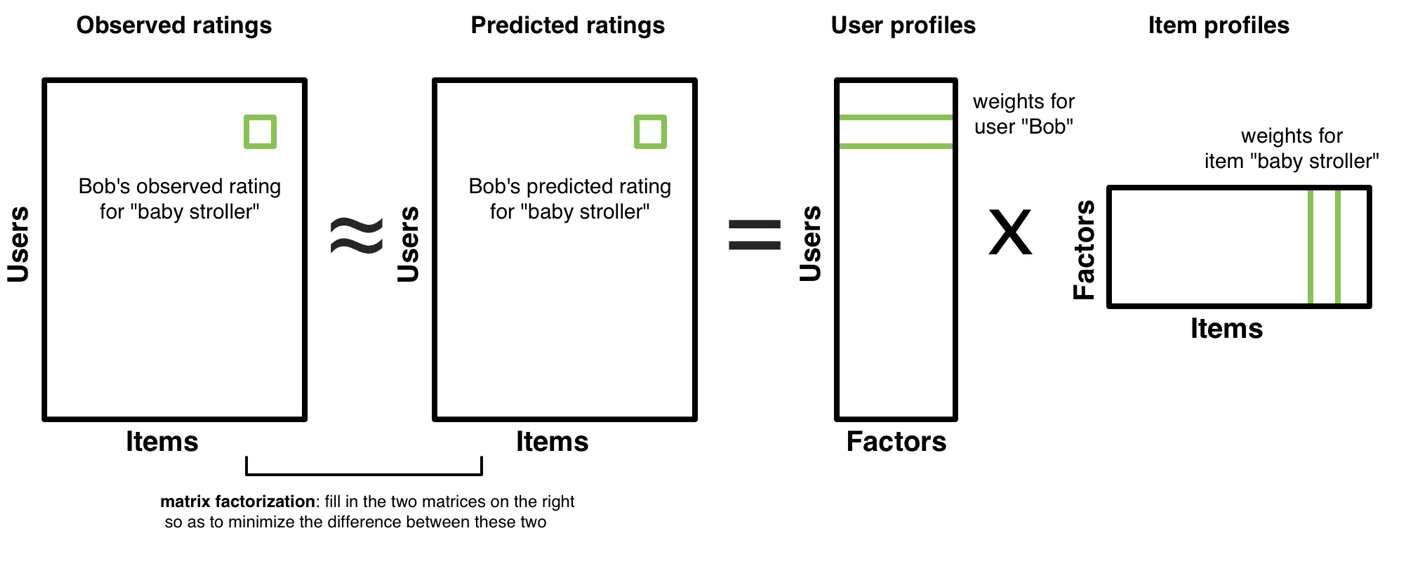
\includegraphics[scale=0.6]{images/mf.png}
\caption{基于矩阵分解的协同过滤算法}
\label{fig:mf}
\end{figure}

如图\ref{fig:mf}所示,第一个矩阵代表原始的大型稀疏矩阵,其中包含已观察到的评分数据和待预测的评分数据,
第三个和第四个矩阵代表用户因子矩阵和电影因子矩阵,在矩阵分解训练的过程中,
我们使两个子矩阵相乘的结果尽可能地去接近原始矩阵中已观察到的评分数据,而不去关心待预测的评分数据,
从而通过原始矩阵生成出这两个子矩阵。第二个矩阵代表生成完两个子矩阵后,两个子矩阵再相乘还原出来的预测矩阵,
该预测矩阵和原始矩阵大小相同,对应的评分位置上,已观察的评分数据和原始矩阵十分接近,
待预测的评分数据也计算出来相应的预测结果,评分预测的任务也自然得到了解决。

具体的训练过程中,我们首先随机初始化用户子矩阵和电影子矩阵,然后定义如下的优化目标:
\begin{equation}
\min_{q*, p*} \sum_{(u, i) \in \mathcal{K} }{ (r_{ui} - q_i^T \cdot p_j)^2 + \lambda (|q_i|^2 + |p_j|^2) }
\end{equation}
其中$\mathcal{K}$代表已观察到的评分数据集合,$r_{ui}$代表观察到的用户$u$给电影$j$的评分数据,
$q_i^T \cdot p_j$代表两个子矩阵相乘后对应的预测评分数据,$\lambda (|q_i|^2 + |p_j|^2)$是保证算法鲁棒性的正则化项。
从该公式我们可以看出,优化目标是使得两个子矩阵的乘积在已观察评分数据上和原始矩阵的差值尽可能的小。
一般会采用随机梯度下降进行算法训练,具体的更新公式为:
\begin{equation}
e_{ui} = r_{ui} - q_i^T \cdot p_u
\end{equation}
\begin{equation}
q_i \leftarrow q_i + \gamma \cdot (e_{ui} \cdot p_u - \lambda \cdot q_i)
\end{equation}
\begin{equation}
p_u \leftarrow p_u + \gamma \cdot (e_{ui} \cdot q_i - \lambda \cdot p_u)
\end{equation}

\subsection{混合的推荐系统}
由于不同的推荐算法各有利弊,所以在实际的应用场景中,单纯一种推荐策略往往并不能满足推荐需求。
工业界的具体实现中,人们常常将多个方法进行混合,从而达到更好的推荐效果。
关于如何混合不同的推荐策略,这里简单地描述几种比较流行的混合方法。
\begin{itemize}
\item \textbf{加权的混合:}
参考集成学习(Ensemble Learning)的思想,使用若干不同的推荐算法获得多个推荐结果,
然后使用线性结合的方式将这些推荐结果按照一定权重组合起来,最后按照新的权重进行重排序,
产生新的推荐列表。这里的具体权重的数值需要在训练数据集上反复试验,从而达到最好的混合推荐效果。
\item \textbf{分层的混合:}
加权的混合策略可以看成是对多个推荐算法的并联处理,同样我们也可以选择串联处理,
将一个推荐方法的输出作为另外一个推荐方法的输入,以此类推,构成一个串联结构,
从而综合各个推荐策略的优缺点,得到更加准确的推荐结果。
\item \textbf{切换的混合:}
除了将多个推荐模型混合在一起,我们也可以选择在不同的生产环境下选择最适应当前情况的推荐方法。
例如,在商品推荐的场景下,如果发现用户数量超过物品数量,我们可以选择使用基于物品的协同过滤算法,
而当物品数量超过用户数量时,我们切换至基于用户的协同过滤算法。
\item \textbf{分区的混合:}
另外,我们也可以在推荐结果展示界面做文章。采用多种推荐机制,将不同的结果分在不同的区域展示给用户。
例如,亚马逊、淘宝和京东等很多电子商务网站都是采用这样的方式,
用户可以得到很全面的推荐,也会更加容易找到他们想购买的商品。
\end{itemize}

\section{推荐系统的评价}
一个完整的推荐系统一般包含两个参与者:用户和物品。以电影推荐为例,
首先推荐系统需要满足用户的需求,为用户推荐其可能喜爱的电影,
其次,推荐系统也需要满足物品的需求,保证各个电影都有被推荐的机会。
一个良好的推荐系统需要同时考虑两者的利益,构成双方共赢的场面。

在推荐系统中,主要存在三种评价推荐效果的实验方法:离线实验、在线实验和用户调查。

离线实验首先通过日志系统获取用户的行为数据,生成一个标准的数据集,
然后按照一定规则将其切分为训练集和测试集,实验者在训练集上训练推荐模型,
并在测试集上进行预测,最后通过离线评价算法得出推荐模型的预测效果。
离线实验不需要一个实际的系统和真实的用户进行验证,可以进行直接快速的计算,
从而方便进行大量的算法验证,是研究人员的首选方案。
但是离线实验无法得出很多商业模式上关心的点击率和转换率等指标。

在线实验又可以称为AB测试,它通过一定规则将在线用户随机分为两组,
一组采用原始的推荐算法,另外一组使用待验证的推荐算法,
通过统计两组用户的点击率和转化率可以对比待验证算法和原始推荐算法的优劣。
在线测试可以公平地获取不同算法实际在线时的性能指标,
但是其成本开销较大,且必须进行长期的实验才能得到可靠的效果,
不太适用于学术界的研究钻研。

用户调研是随机招募一些真实用户,让他们在待测试的推荐系统上完成一些任务,
实验者观察并记录用户行为,最后让用户回答一些问题,
通过用户行为和用户答案我们可以获知待测试推荐系统的性能。
用户调研需要保证分布真实,比如男女各半,还需要进行双盲实验。
用户调研可以直观得出用户使用过程中的感受,
缺点是很难进行大规模的验证,统计意义不足,容易出现较大的效果偏差。

由于推荐系统应用场景的多样性,历史上研究人员提出了多种评价推荐系统性能的指标,
有些指标可以定量计算,有些只能定性描述。我们下面简单介绍其中有名的几类。

\subsection{用户满意度}
用户满意度是用户对推荐系统效果最直观的评价,其无法通过里县实验计算,
只能通过在线实验或者用户调研获得。
在线实验中,用户满意度一般和用户行为挂钩,
我们既可以在推荐结果列表里添加满意和不满意两种按钮供用户进行直接反馈,
也可以通过点击率,停留时间和转化率等指标进行衡量。
用户调研中,用户满意度一般和用户答案挂钩,
通过设计问卷调查题目,我们可以了解用户对当前推荐系统各个方面的满意程度。

\subsection{预测准确度}
预测准确度是离线实验中最重要的评价指标,其度量推荐系统预测用户未来行为的能力,
主要分为两种:评分预测和TopN预测。

\begin{itemize}
\item \textbf{评分预测}
推荐系统的很多应用场景中,都提供了用户给物品进行评分的功能,
通过评分数据可以反应用户对物品的偏爱程度。
通过用户的历史评分数据,实验者建立推荐模型,预测用户将来的评分数据,
系统系统可以选择其中评分较高的物品进行推荐。
评分预测的预测准确度一般通过均方根误差(Root Mean Square Error, RMSE)
和平均绝对误差(Mean Absolute Error, MAE)计算。
对于测试集T中的每一个用户$u$和物品$i$,假设$r_{ui}$代表用户$u$对于
物品$i$的真实评分,$\hat{r}_{ui}$代表推荐算法的预测评分,
则均方根误差的计算公式为:
\begin{equation}
RMSE = \sqrt{\frac{\sum_{u,i \in T}{(r_{ui} - \hat{r}_{ui})^2}}{|T|}}
\end{equation}
平均绝对误差的计算公式为:
\begin{equation}
MAE = \frac{\sum_{u,i \in T}{|r_{ui} - \hat{r}_{ui}|}}{|T|}
\end{equation}
对比均方根误差和平均绝对误差,
Netflix认为均方根误差加大了对预测不准的评分的惩罚(平方项的惩罚),
因此均方根误差相对平均绝对误差更加苛刻。

\item \textbf{TopN预测}
推荐系统的展示结果一般是一个包含若干物品的个性化推荐列表,我们一般称之为TopN推荐,
其预测准确率一般通过对比个性化推荐物品列表和用户真实喜爱物品列表,
计算准确率(Precision)和召回率(Recall)来实现。
对于测试集T中的每一个用户$u$,假设$R(u)$代表用户$u$真实喜爱的物品列表,
而$\hat{R}(u)$代表推荐给用户$u$的个性化推荐列表,
则准确率的计算公式为:
\begin{equation}
Precision = \frac{ \sum_{u \in T}{|R(u) \cap \hat{R}(u)|} }{ \sum_{u \in T}{|\hat{R}(u)|} }
\end{equation}
召回率的计算公式为:
\begin{equation}
Recall = \frac{ \sum_{u \in T}{|R(u) \cap \hat{R}(u)|} }{ \sum_{u \in T}{|R(u)|} }
\end{equation}
\end{itemize}
准确率体现了在我们推荐的物品列表里面,用户喜爱的占比多少。
而召回率体现了在用户喜爱的物品列表里面,我们推荐的占比多少。
两者都是数值越大,推荐效果越好。
同时,我们也会使用$F1$值来结合准确率和召回率,其计算公式为:
\begin{equation}
F1 = \frac{Precision \cdot Recall}{ \alpha \cdot Precision + (1 - \alpha) \cdot Recall }
\end{equation}
其中,$\alpha$的数值位于0到1之间,用于控制准确率和召回率两者相对的影响因子。

\subsection{其他指标}
同时推荐系统中还包含其他一些评价指标,我们在此简单介绍如下:
\begin{itemize}
\item \textbf{覆盖率}描述了一个推荐系统对长尾物品(Long Tail)的挖掘能力,
可以简单定义为所有推荐出来的物品占总物品集合的比例。具有较高覆盖率的推荐系统不仅可以推荐热门物品,
还可以推荐少数人喜爱的小众物品。
\item \textbf{多样性}描述了推荐列表中物品两两之间的不相似性,
具有较高多样性的推荐系统尽可能满足用户多种兴趣需求。
\item \textbf{新颖性}代表推荐系统为用户推荐了他们以前没有听说过的物品,
在一个网站实现新颖性的最简单的方式就是过滤掉用户之前有过行为的物品。
\item \textbf{惊喜度}表示推荐系统给用户推荐了和其历史上喜欢的物品不相似的物品,
但是却可以令用户感到满意,是一种定性的度量方式。
\item \textbf{信任度}描述了用户对推荐系统给出的推荐结果的信任程度,
具有解释性的推荐结果一般具有较高的信任度。
\item \textbf{实时性}保证推荐系统可以实时地更新推荐列表来满足用户新的行为的变化,
也需要推荐系统能够将新加入推荐平台的新物品可以推荐给用户。
\item \textbf{健壮性}代表推荐系统的抗攻击能力,常见的攻击手段是注入攻击,
利用大量的虚假账号来为自己的物品评非常高的分数,从而欺骗推荐系统。
\end{itemize}

\section{深度学习在自然语言处理中的成功应用}
\subsection{词向量表示}
早期的词向量表示是独热表示法(One-Hot Representation),在高维向量中只有一个维度描述了词语的信息,
没有词序信息,也无法准确地捕捉语义信息,存在严重的``语义鸿沟''现象。例如``卡拉OK''和``麦克风''
在语义上指代同一件物品,但是在独热表示中却无法观察得到。
Hinton等人\parencite{hinton1986learning}在1986年提出分布表示法(Distributed Representation),
其基本思想是 通过训练将每个词映射成$K$维实数向量,
通过向量之间的距离(余弦相似度或欧氏距离等)来判断它们之间的语义相似度。
这样以来,``卡拉OK''和``麦克风''就可以映射到两个距离很近的低维实数向量中,从而体现两者语义相近的关系。

Word2Vec是谷歌公司在2013年开源的一款将词映射为实数向量的高效工具,由Mikolov等人\parencite{mikolov2013efficient}提出。
其利用深度学习的思想,可以通过训练把对文本内容的处理简化为低维实数向量空间中的向量运算,
而向量空间上的相似度可以用来表示文本语义上的相似度。同时,输出的词向量是连续的向量,可以支持使用连续模型做文本处理。
Word2vec输出的词向量可以被用来做很多自然语言处理相关的工作,比如文本聚类、词性分析、机器翻译等等。
训练出的向量有一定的特性,即相近意义的词在向量空间上其距离也是相近,
有一个经典例子就是$V(`king') – V(`man') + V(`woman') \approx V(`queen')$。

Word2Vec是一个用于处理文本的双层神经网络,它的输入是大量的文本语料,输出则是每个词语对应的一个向量表示,
主要包括两个基本模型:CBOW模型和Skip-gram模型。其中CBOW模型使用上下文预测目标词,
而Skip-gram模型则是用一个词来预测一段上下文。

\begin{figure}[htbp]
\centering
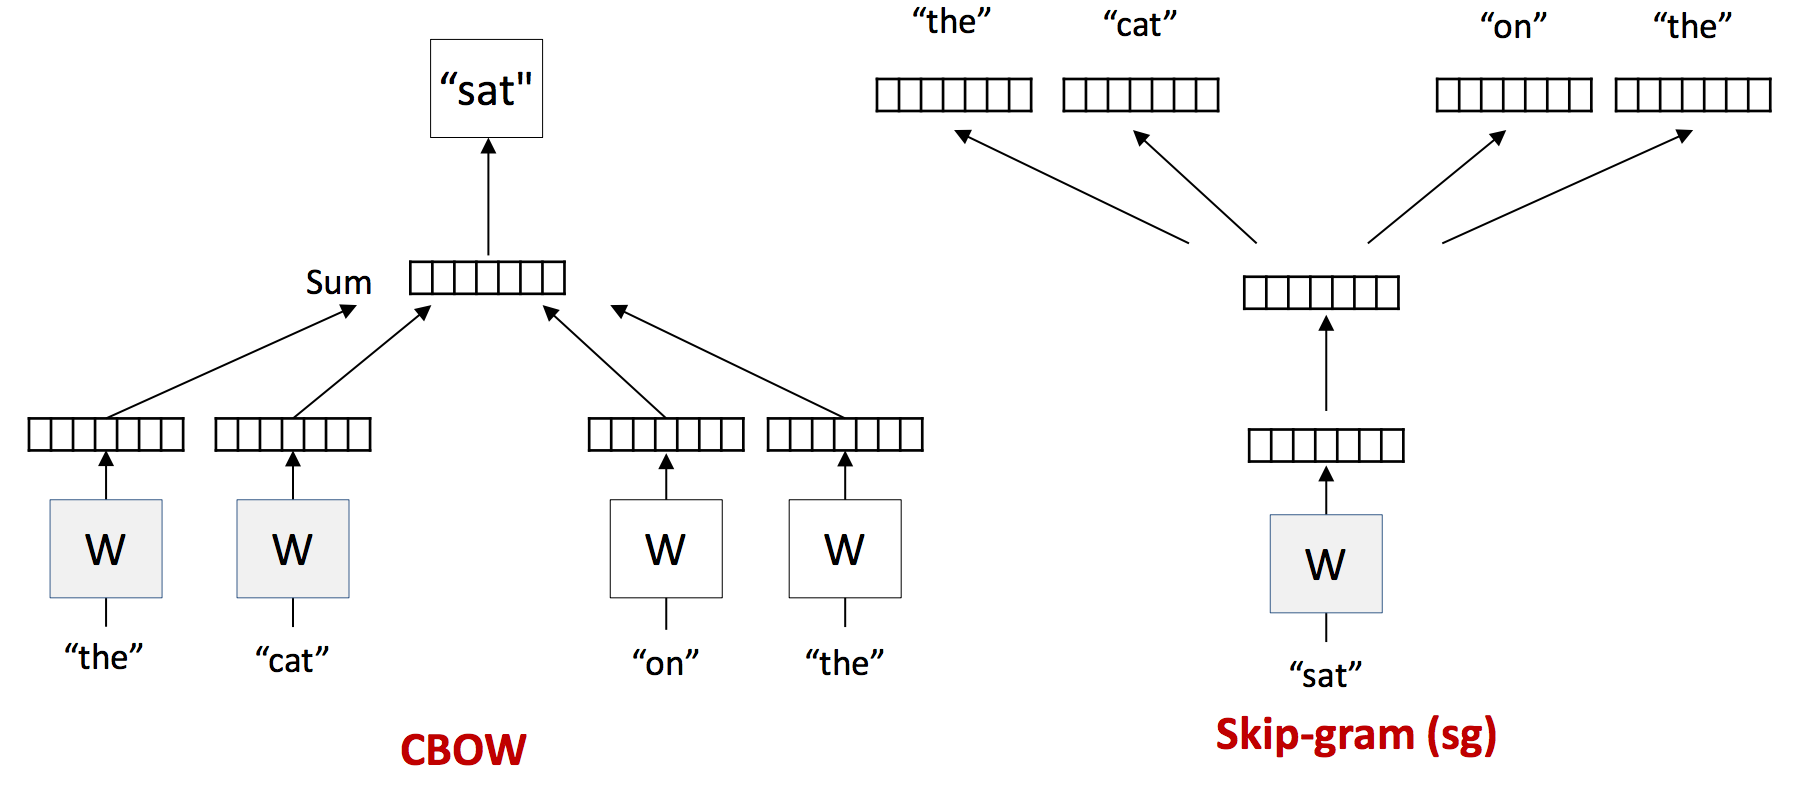
\includegraphics[scale=0.4]{images/w2v.png}
\caption{Word2Vec中的CBOW模型和Skip-gram模型示意图}
\label{fig:word2vec}
\end{figure}

图\ref{fig:word2vec}展示了CBOW模型和Skip-gram模型的示意图,左半部分代表CBOW模型,
``the'', ``cat'', ``on''和``the''是一个语义窗口内的上下文,``sat''是目标词,
每个词语会被赋予一个长度为$K$的随机初始化的向量进行表示,上下文通过聚合的方式形成一个整体,
然后对目标词进行预测,预测过程中的误差会被反向传播回来对上下文的词向量进行更新,直到最后收敛,
从而完成训练过程。具体来说,CBOW模型的目标函数是:
\begin{equation}
Loss = \sum_{t=1}^T {\log P(w_t| w_{t-c} : w_{t+c}) }
\end{equation}
这里的$T$代表训练语料中的所有词语的数量,$c$表示上下文的窗口大小,$w_{t-c} : w_{t+c}$除了$w_t$本身的上下文序列。
似然概率$P(w_t| w_{t-c} : w_{t+c})$使用softmax定义,上下文序列的聚合可以使用向量和或者向量均值来实现。

右半部分代表Skip-gram模型,和CBOW模型不同的是,其使用当前词语来预测上下文,
``sat''是当前词,``the'', ``cat'', ``on''和``the''是一个语义窗口内的上下文,
同样地,每个词语会被赋予一个长度为$K$的随机初始化的向量进行表示,当前词语作为输入对上下文中的所有词语进行预测,
预测过程中的误差会被反向传播回来对当前词语的词向量进行更新,直到最后收敛,从而完成训练过程。
具体来说,Skip-gram模型的目标函数是:
\begin{equation}
Loss = \sum_{t=1}^T {\log P(w_{t-c} : w_{t+c} | w_t) }
\end{equation}
这里的$T$代表训练语料中的所有词语的数量,$c$表示上下文的窗口大小,$w_{t-c} : w_{t+c}$除了$w_t$本身的上下文序列。
似然概率$P(w_{t-c} : w_{t+c} | w_t)$也是使用softmax定义.

\subsection{句向量表示}
2014年Le等人\parencite{le2014distributed}在Word2Vec的基础上提出了Doc2Vec模型,其原理与Word2Vec非常的相似。
Doc2Vec也包括两个基本模型,分别是DM模型和DBOW模型,如图\ref{fig:doc2vec}所示。

\begin{figure}[htbp]
\centering
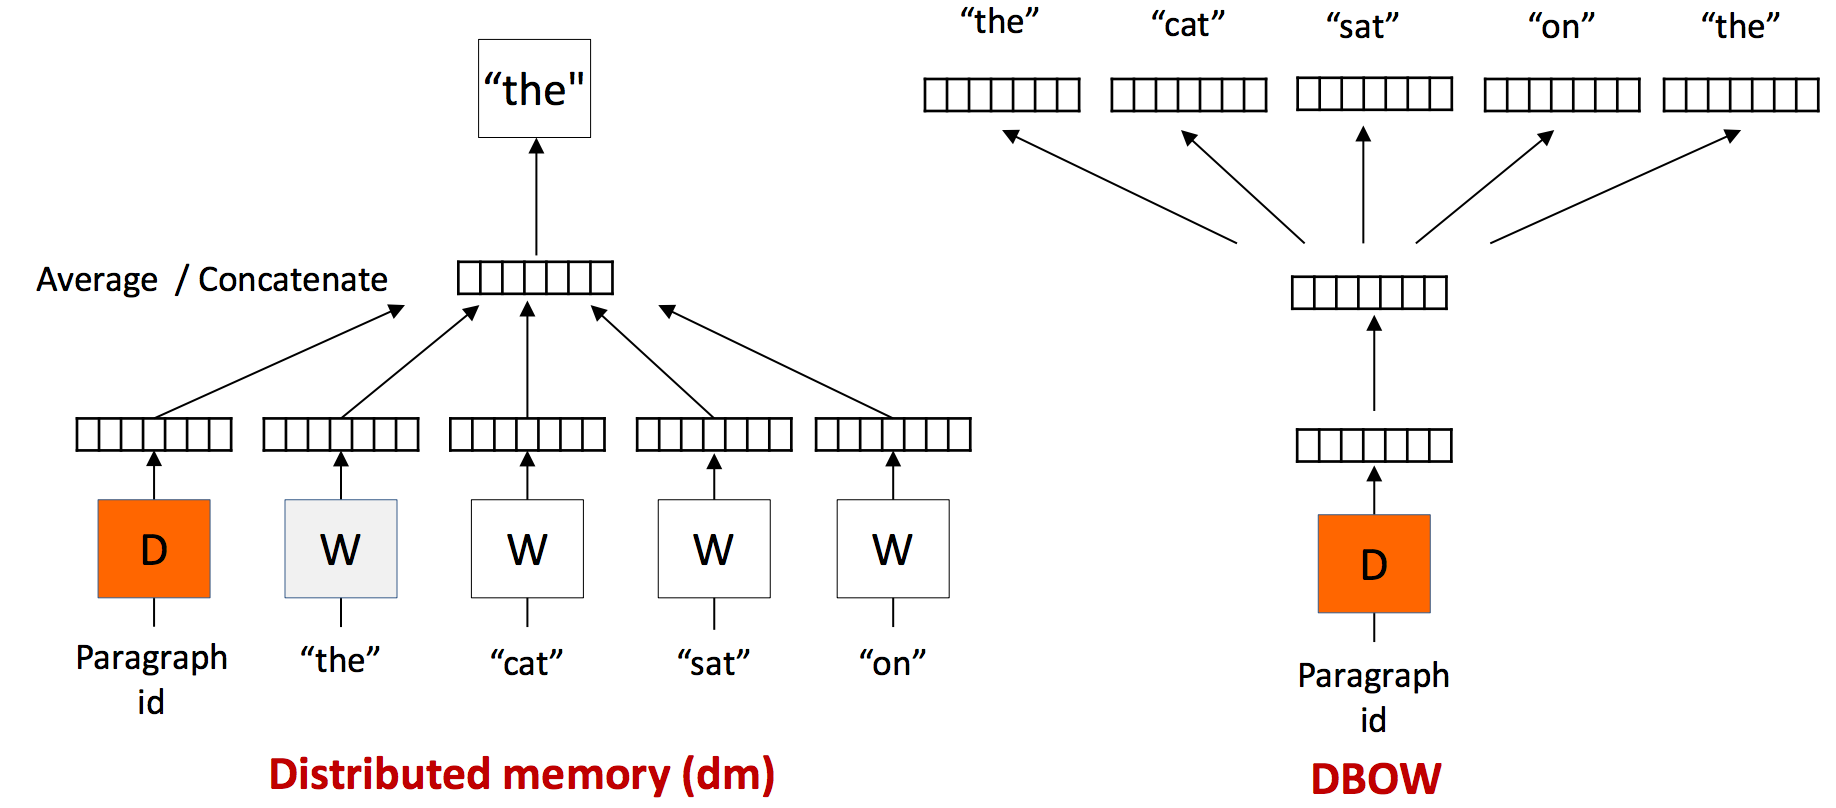
\includegraphics[scale=0.4]{images/d2v.png}
\caption{Doc2vec中的DM模型和DBOW模型示意图}
\label{fig:doc2vec}
\end{figure}

可以看出DM模型和CBOW模型方法类似,DBOW模型和Skip-gram模型方法类似。
不同于Word2Vec的是,Doc2Vec在整个模型中引入了句向量表示,即每一个句子也拥有一个向量表示。
图中的左半部分是DM模型,其在使用上下文预测目标词的同时额外加上了一个全局的句子向量作为输入信息,
而右半部分是DBOW模型,使用句子向量去预测上下文。
因为Doc2Vec算法和Word2Vec算法十分类似,这里不再赘述。

\section{深度学习在推荐系统中的成功应用}
自从深度学习在语音识别和图像识别领域取得突破性进展后,不少研究领域开始尝试在自己领域中引入深度学习,
推荐系统也不例外,在本章节中我们会从自动编码机和循环神经网络两个模型出发介绍深度学习在推荐系统中的成功应用。

\subsection{自动编码机}
自动编码机(Autoencoder)是一种特殊的神经网络结构,最简单的自动编码机由三层网络组成,
分别是输入层,隐藏层和输出层。其中输入层神经元数量与输出层神经元数量相等,隐藏层神经元数量少于输入层和输出层。
自动编码机的训练目标是是的输出信息和输入信息尽可能相似,因为隐藏层神经元数量较少,
所以在数据从输入层到隐藏层的过程可以看成是一种压缩行为,也可以理解为对输入数据的一种编码过程;
而从隐藏层到输出层可以看成数据的解压缩行为,也可以理解为对隐藏层数据的一种解码过程。
因为隐藏层瓶颈的存在,迫使自动编码机学习了对原始输入数据进行压缩提取的一个过程。

Sedhain等人\parencite{sedhain2015autorec}最早提出使用自动编码机通过重构评分数据的方式直接进行评分预测,
Strub等人\parencite{strub2016hybrid}在此基础上进行了改进,
提出了如图\ref{fig:ae}所示的CFN(Collaborative Filtering Neural network)模型,
将噪音去除机制引入训练过程中,极大增强了整个模型的鲁棒性,

\begin{figure}[htbp]
\centering
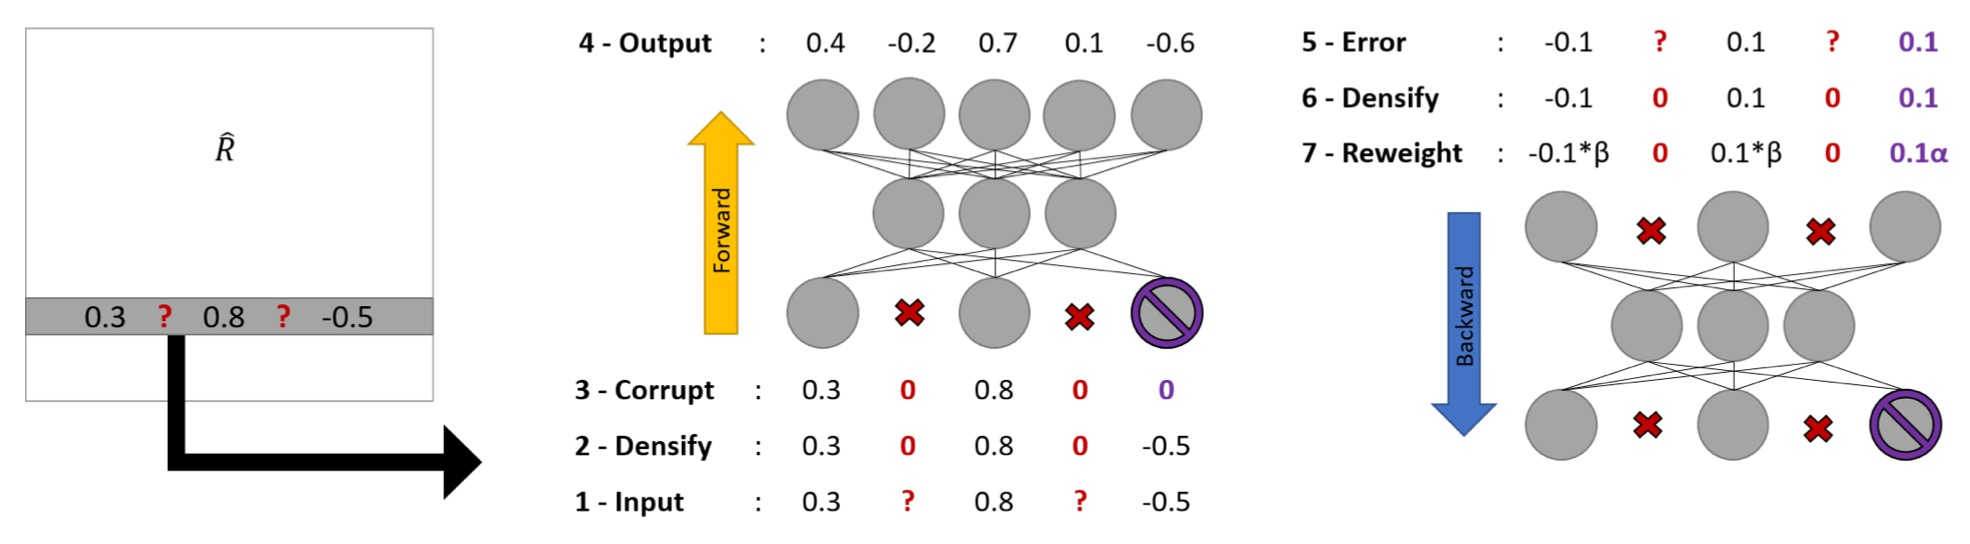
\includegraphics[scale=0.22]{images/ae.jpeg}
\caption{自动编码机}
\label{fig:ae}
\end{figure}

图中的左边部分代表原始的大型稀疏矩阵,CFN模型会对其中的数据进行分行处理,
即将每一个用户的所有评分作为一个样本输入进自动编码机中。
如果从物品的角度出发,CFN模型就会进行分列处理,将每一个物品的所有评分作为一个样本输入进自动编码机中。
图中的中间部分表示CFN模型的正向传播过程。评分数据主要分为已观察到的评分和待预测的评分两类。
对于已观察到的评分,CFN模型会以一定的概率将其变成噪声数据,如图中的紫色节点表示的``-0.5''分被变成了噪声数据``0''分;
对于待预测的评分数据,CFN模型会将其进行标记,从而在训练优化过程中将其忽略,如图中的红色叉型节点。
图中的右边部分代表CFN模型的误差反向传播过程,对于待预测的评分CFN模型将其从误差函数中去除,
对于已观察到的数据,分为是否是噪声数据进行不同权重的误差累计,
图中紫色节点的误差被乘以系数$\alpha$作为修改后的误差,而灰色节点的误差被乘以系数$\beta$作为修改后的误差,
红色节点的误差则被忽略。

通过这样的过程,CFN模型利用自动编码机从输入数据中重构出那些被变成噪声数据的评分,
从而学习出不同用户评分数据之间的关系。完成训练后,我们可以将输出层中的待预测评分数据作为预测结果。
另外图中的自动编码是只包含一个隐藏层,CFN模型还可以增加网络的深度,学习出更加深层的数据关系。
最后,CFN还提出了在输入层加入辅助信息的方式来减缓推荐系统中的冷启动问题,
实验结果证明加入辅助信息对评分较少的用户和物品都有较大的预测准确度提升。

CFN模型和本文方法都是使用定制的神经网络结构对推荐问题进行建模,不同的是他们采用了自动编码机,而我们使用了多层感知器。
相比较而言,相同实验设定下,自动编码机模型的参数规模大约是多层感知器的两倍,主要因为自动编码机包含编码层和解码层,
而多层感知器只有编码层;但由于噪声机制的引入,CFN模型除了具备数据还原能力和数据去噪能力,
在预测准确度和鲁棒性上都高于多层感知器。

\subsection{循环神经网络}
循环神经网络是一种特殊的神经网络结构,在处理序列数据上有着其得天独厚的优势,通过隐藏层节点保存历史序列信息,
并在每次迭代中融入新的信息,从而完成序列标注,分类预测等任务。
循环神经网络并不能很好地处理较长的序列,一个改进版本的循环神经网络是LSTM(Long Short Term Memory),
通过加入输入门、遗忘门和输出门,LSTM可以刻画较长序列中的远距离依赖问题。

\begin{figure}[htbp]
\centering
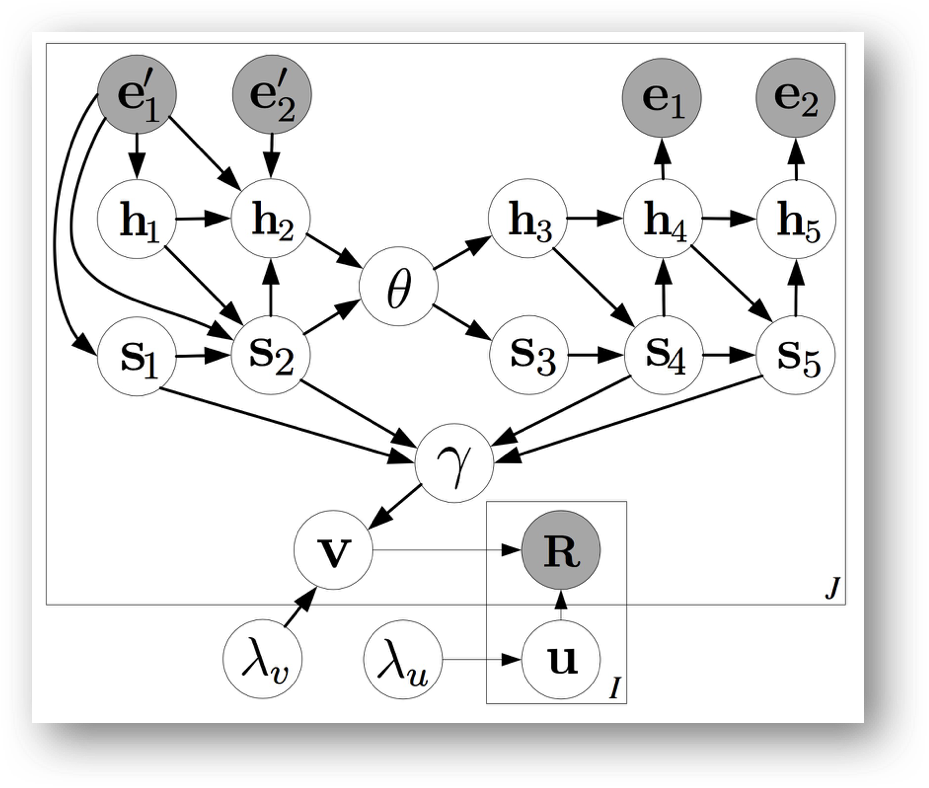
\includegraphics[scale=0.6]{images/pmf_rnn.png}
\caption{循环神经网络}
\label{fig:pmf_rnn}
\end{figure}

循环神经网络在很多自然语言处理任务中取得了巨大成功以及广泛应用,例如文本分类,机器翻译,对话模型等等。
Wang等人\parencite{wang2016collaborative}提出贝叶斯版本的循环神经网络来对论文摘要文本信息进行提取,
然后将其加入到概率矩阵分解中,在论文推荐任务中取得优异的性能表现,整个算法框架如图\ref{fig:pmf_rnn}所示。

图中上半部分表示循环神经网络对论文摘要信息进行提取,其中``e''节点代表文本信息中的一个个单词,
``h''节点和``s''节点分别代表LSTM中的隐藏节点和状态节点,在该网络结构中,
循环神经网络首先接受一段文本输入,逐步将每个单词信息编码进隐藏节点和状态节点中,
然后通过中间的一个瓶颈节点``$\theta$''进行压缩和解压缩,再逐步将每个单词信息解码输出出来。
这是一个典型的``seq-to-seq''框架,通过重构本身数据的方式将文本信息融入到神经网络的节点中。
紧接着,使用``$\gamma$''节点聚合了所有的隐藏节点和状态节点信息,这里可以看成是加权求和,
然后综合``$\lambda_v$''节点生成了``$v$''节点,即物品节点。
最后物品节点``$v$''和用户节点``$u$''进行组合,得到评分节点``$R$''。
整个框架中,所有的灰色节点是已知数据,即评分数据和文本信息,所有的白色节点是待学习的数据,
包括用户节点和物品节点等。因为是贝叶斯网络结构,所以训练过程通过最大后验概率实现。

相对于传统的词袋模型,Wang等人提出的方法中的循环神经网络可以更好地刻画文本数据之间的序列关系,
从而保证学习出来的文本信息更加地准确和丰富,多项实验结果也证明了该算法的有效性。
和Wang等人工作不同的是,我们并没有利用这些文本信息数据,而是利用用户的评分时间信息对物品相似度进行建模。
Wang等人的工作可以看成是基于内容的方法的一种实现,本文的工作则是基于协同过滤的方法的一种实现。
在文本信息较为丰富的场景下,如论文推荐、图书推荐等,Wang等人的工作更加具备优势,
而在文本信息较为稀缺的场景下,如商品推荐、音乐推荐等,我们的工作则更加适用。


